%----------------------------------------------------------------------------------------
%	PACKAGES AND OTHER DOCUMENT CONFIGURATIONS
%----------------------------------------------------------------------------------------

\documentclass[
12pt, % The default document font size, options: 10pt, 11pt, 12pt
oneside, % Two side (alternating margins) for binding by default, uncomment to switch to one side
chapterinoneline,% Have the chapter title next to the number in one single line
english, % ngerman for German
onehalfspacing, % Single line spacing, alternatives: onehalfspacing or doublespacing
%draft, % Uncomment to enable draft mode (no pictures, no links, overfull hboxes indicated)
nolistspacing, % If the document is onehalfspacing or doublespacing, uncomment this to set spacing in lists to single
%liststotoc, % Uncomment to add the list of figures/tables/etc to the table of contents
%toctotoc, % Uncomment to add the main table of contents to the table of contents
%parskip, % Uncomment to add space between paragraphs
%nohyperref, % Uncomment to not load the hyperref package
headsepline, % Uncomment to get a line under the header
]{MastersDoctoralThesis} % The class file specifying the document structure

\usepackage{cmap}

\usepackage[utf8]{inputenc} % Required for inputting international characters
\usepackage[T2A]{fontenc} % Output font encoding for international characters

\usepackage[backend=bibtex,style=numeric,natbib=true]{biblatex} % Use the bibtex backend with the authoryear citation style (which resembles APA)

\addbibresource{references.bib} % The filename of the bibliography

\usepackage[autostyle=true]{csquotes} % Required to generate language-dependent quotes in the bibliography

\usepackage{wrapfig}
\usepackage{float}

\usepackage{caption}
\captionsetup[table]{name=Таблица}
\captionsetup[figure]{name=Фигура}

\usepackage{longtable}

\usepackage{indentfirst}

\usepackage{pgfplots}
\pgfplotsset{
	width=12.5cm,
    compat=1.9,
    height=7.5cm,
	xlabel={Номер на итерация},
    ylabel={Точност в \%},
    xmin=1, xmax=25,
    ymin=0, ymax=100,
    xtick={1,5,10,15,20,25},
    ytick={0,20,40,60,80,100},
    legend style={at={(0.5,-0.2)},anchor=north},
    legend cell align=left,
    ymajorgrids=true,
    grid style=dashed,}
    
\usepackage{microtype}

%----------------------------------------------------------------------------------------
%	MARGIN SETTINGS
%----------------------------------------------------------------------------------------

\geometry{
	paper=a4paper, % Change to letterpaper for US letter
	inner=2.5cm, % Inner margin
	outer=3.8cm, % Outer margin
	bindingoffset=2cm, % Binding offset
	top=1.5cm, % Top margin
	bottom=1.5cm, % Bottom margin
    head=29pt,
	%showframe,% show how the type block is set on the page
}

%----------------------------------------------------------------------------------------
%	THESIS INFORMATION
%----------------------------------------------------------------------------------------

\hypersetup{pdftitle=Автоматично разделяне на големи количества изображения на класове с използване на дълбоко учене (deep learning)} % Set the PDF's title to your title
\hypersetup{pdfauthor=Валентин Змийчаров} % Set the PDF's author to your name

\begin{document}
\sloppy

%\frontmatter % Use roman page numbering style (i, ii, iii, iv...) for the pre-content pages

\mainmatter % Begin numeric (1,2,3...) page numbering

\pagestyle{thesis} % Default to the plain heading style until the thesis style is called for the body content

%----------------------------------------------------------------------------------------
%	TITLE PAGE
%----------------------------------------------------------------------------------------

\begin{titlepage}
\begin{center}

\Large \textbf{Софийски университет \\ „Св. Климент Охридски”}\\[0cm]
\Large Дипломна работа\\[0cm]
\Large \textit{Катедра „Софтуерни технологии”}\\[0.2cm]


\includegraphics{Figures/logo_su.jpg}

\includegraphics{Figures/logo_katedra.jpg}\\[0.1cm]

\HRule \\[0.1cm] % Horizontal line
{\huge \bfseries Автоматично разделяне на големи количества изображения на класове с използване на дълбоко учене (deep learning)\par}\vspace{0.1cm} % Thesis title
\HRule \\[0.2cm] % Horizontal line
 
\begin{flushleft} \large
Дипломант:\\ \textbf{Валентин Змийчаров}\\
Специалност:\\ \textbf{Извличане на информация и откриване на знания}\\
Факултетен номер:\\ \textbf{24952} \\
Научен ръководител:\\ \textbf{Д-р Милен Чечев}\\[0.2cm]
\end{flushleft}

{\large София 2017г.}\\
 
\vfill
\end{center}
\end{titlepage}

%----------------------------------------------------------------------------------------
%	LIST OF CONTENTS/FIGURES/TABLES PAGES
%----------------------------------------------------------------------------------------

\renewcommand{\contentsname}{Съдържание}
\tableofcontents % Prints the main table of contents

%----------------------------------------------------------------------------------------
%	THESIS CONTENT - CHAPTERS
%----------------------------------------------------------------------------------------


% \pagestyle{thesis} % Return the page headers back to the "thesis" style

\chapter{Увод}

\label{Chapter1}

%----------------------------------------------------------------------------------------

\section{Актуалност на проблема и мотивация}

Разпознаването на изображения е способност на човека, която не е тривиално да бъде решена от компютър. Класифициране на изображения означава причисляване на изображение към един или повече класове с определена точност. Нека например имаме непресичащи се класове за превозни средства: автомобил, мотор, самолет, кораб, подовдница. Нека имаме изображенията, показани на \ref{fig:example_images}.\\[0.5cm]

\begin{figure}[h!]
\centering
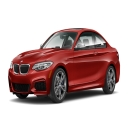
\includegraphics[width=115px,height=100px]{Figures/car.jpg}
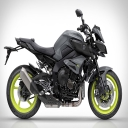
\includegraphics[width=115px,height=100px]{Figures/motorcycle.jpg}
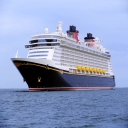
\includegraphics[width=115px,height=100px]{Figures/ship.jpg}
\caption{Примерни изображения}
\label{fig:example_images}
\end{figure}

Целта е първата картинка да се причисли към класа автомобили, втората към класа мотоциклети и третата към кораби. Това е елементарно за човешкото око, но компютърът вижда само последователност от нули и единици. Освен това при дадения пример разликите са големи, но може да се налага да се класифицират изображения, които са трудно различими дори с просто око.

Проблемът е особено актуален, поради непрестанното използване на социални мрежи и облачни услуги в световен мащаб. Всеки ден над 350 милиона снимки се качват само във Facebook \cite{FacebookFacts}. С използване на модерните технологии заснемаме гигантско количество изображения и много често след това просто забравяме за тях. Непосилна задача е ръчно да обозначим съдържанието на всяка една от снимките. Тук на помощ идва автоматичната обработка и анализ на съдържанието на изображения.

С намирането на добро решение на проблема са се захванали някои от най-големите компании в сферата на информационните технологии:

\begin{itemize}
\item \textbf{Google photos} \cite{GooglePhotos} използва автоматично класифициране на изображения, за да групира снимките, които качваме по категории и папки. Огромна публичност доби скандал с автоматичното категоризиране, при който двойка тъмнокожи бяха категоризирани като горили \cite{GoogleGorillas}. Това повдигна редица етични въпроси относно проблема. Google също предоставя и API за категоризация на изображения: Vision API \cite{GoogleVisionAPI}, което позволява интегрирането на софтуер за разпознаване на изображения в собствена система.
\item \textbf{Microsoft} също предоставя подобна услуга за своите облачни услуги. Те имат и аналогично API \cite{MicrosoftVisionAPI}.
\item Amazon, Dropbox също поддържат подобни услуги, което говори за потенциала на разпознаването на изображения.
\end{itemize}

Бизнесът на някои компании изцяло лежи на разпознаването на изображения. Такива са Imagga \cite{Imagga}, Clarifai \cite{Clarifai}.

Предоставянето на тази функционалност като услуга за бизнесите предразполага раждането на много оригинални идеи. Такива са вече споменатите облачни услуги. С наличието на API за разпознаване на изображения всеки доставчик на облачни услуги може да направи автоматична категоризация на изображенията на потребителите. Друг интересен случай са сайтове и приложения за споделяне на авторски изображения. При тях обемът на данните е огромен и в повечето случаи няма никаква конкретна информация.

Разпознаването на обекти в изображението би могло да бъде от полза и по отношение на сигурността. При голямо количество съдържание може лесно да се намерят например оръжия или снимки с нецензурирано съдържание. Обемът на снимките расте с гигантски размери и е единствено въпрос на въображение от страна на компаниите какви ползи могат да се извлекат от автоматичното категоризиране на изображения.

\section{Цел и задачи на дипломната работа}
Целта на дипломната работа е да проучи съвременните подходи за класифицирането на изображения, като се дават детайли за използването на конволюционни невронни мрежи с дълбоко обучение.

Задачите биха могли да се обобщят по следния начин:
\begin{enumerate}
\item Обзор на проблемната област. Да се направи проучване на различните софтуерни платформи, които може да се използват за класифициране на изображения в големи мащаби. Какви са предимствата и недостатъците на всяка една от тях. Какво използват най-големите компании в тази сфера.
\item Какви са условията (финансови, хардуерни и др.), за да построим класификатор с добра точност. Какво е добра точност и каква точност постигат готовите решения.
\item Подбор на данни за обучение. Намиране на достатъчно голям обем категоризирани изображения с добро качество с цел обучение.
\item Реализация на прототип за класификация на изображения.
\item Експерименти за оценка на точността на класификацията и възможностите за работа с големи данни.
\item Анализ на получените резултати.
\end{enumerate}

\section{Структура на дипломната работа}

Глава 1 е въведение в проблемната област. Тя цели да покаже кратко каква е целта на дипломната работа и мотивацията да се разреши точно този проблем. Обсъдени са резултатите, които трябва да се постигнат.

Глава 2 представя в детайли използваните алгоритми и подходи. Освен това в нея се аргументира изборът на подход с конволюционни невронни мрежи и се прави подробен анализ на най-доброто решение до момента на писане на дипломната работа.

Глава 3 мотивира избора на технологии, платформи, услуги и библиотеки, които са необходими при разработването на конволюционната невронна мрежа за класифициране на изображения. Направено е въведение в спецификите на Python и Tensorflow като са анализирани различните функционалности и спрямо изискванията на конкретния проблем е избрано подмножество от тях.

Глава 4 дава подробен поглед върху процеса по реализация на конволюционната невронна мрежа за класифициране на изображения и избора на архитектура. Вниманието е насочено към направените експерименти и анализ на резултатите от тях.

Глава 5 е заключителната част, даваща насоки за бъдещо развитие на системата и обобщаващо в каква степен са изпълнени първоначалните поставени цели и задачи. 

\chapter{Преглед на предметната област} % Main chapter title

\label{Chapter2} 

%----------------------------------------------------------------------------------------

\section{Въведение}

През 1959 г. Артър Самюел определя машинното самообучение като „Поле на проучване, което дава на компютрите възможността да учат, без да бъдат експлицитно програмирани“. То изследва проучването и изграждането на алгоритми, които да правят прогнози чрез данни и от които да може да се учи. Машинното самообучение използва събрани исторически данни  за изграждането на модел, който в последствие да може да се използва върху нови данни.

Машинното самообучение се използва в широка гама от изчислителни задачи, където програмирането на експлицитни алгоритми е неосъществимо. Примерните приложения включват филтриране на спам, оптично разпознаване на символи, търсачки и компютърно зрение.

В областта на аналитични данни, машинното самообучение се използва за разработване на сложни модели и алгоритми, които се поддават на прогнозиране. Тези аналитични модели позволяват изследователи, учени и инженери да получават надеждни, повтаряеми решения и резултати.

\section{Разпознаване на изображения: мотивация и история}

През 1963 година в докторската си теза Л. Робъртс \cite{Solids1963} разглежда в детайли как машините могат да възприемат дадени триизмерни обекти от изображение. Той анализира очертанията на обектите и различните перспективи на заснемане. През 1987 година учени от Кеймбридж (Масачузетс) описват разпознаване на обекти с използване на изкуствен интелект \cite{Alignment1987}. Намират се изключително много приложения на разпознаването на обекти в изображения и все повече и повече данни започват да бъдат налични.

В края на 70-те и началото на 80-те невронните мрежи започват да добиват все по-голяма популярност и започват да се прилагат в множество области. Конволюционните невронни мрежи са вдъхновени от зрението на животните в природата. В началото на 21 век се случват няколко много важни неща, които предразполагат развитието на пазара в сферата на автоматичното класифициране на изображения.

Едно от тях е, че се намират начини за използване на видео картата за изчисления в невронните мрежи, което значително подобрява времето на изпълнение. Със създаването и популяризирането на социалните мрежи броят на картинките е огромен: всеки ден над 350 милиона снимки се качват само във Facebook \cite{FacebookFacts}.

Активното използване на автоматично разчитане на изображения се прилага активно в днешни дни. То служи за разпознаване на номера от автомобили, пощенски кодове и чекове. Все с по-голяма сила навлиза разпознаването на пръстови отпечатъци за идентификация \cite{Fingerprints}.

Със особено влияние са алгоритмите за локализиране и разпознаване на лице на хора. При наличието на много улични камери такъв алгоритъм разполага с възможност да търси в гигантско количество информация.

С увеличаването на интернет потребителите се увеличават и заплахите в електронния свят. Публично се разпространяват изображения, свързани с насилие, детска порнография и други нецензурирани материали. Автоматичното разпознаване на изображения идва на помощ при засичането на подобни нередности.


%----------------------------------------------------------------------------------------

\section{Невронни мрежи}

Невронната мрежа е модел за обработка на информация, вдъхновен от изучаването на биоелектричните мрежи в мозъка на човека и животните, образувани от неврони и техните синапси. В наши дни учените често наричат изкуствените невронни мрежи просто невронни мрежи.

Математическият аналог на биологичната невронна мрежа представлява множество от взаимносвързани прости изчислителни елементи (неврони). Всеки неврон приема сигнали от другите (под формата на числа), сумира ги, като сумата минава през активационна функция, и така определя своята активация (степен на възбуда), която се предава по изходящите връзки към другите неврони. Всяка връзка има тегло, което, умножавайки се със сигнала, определя неговата значимост (сила). Теглата на връзките са аналогични на силата на синаптичните импулси, предавани между биологичните неврони. Отрицателна стойност на теглото съответства на потискащ импулс, а положителна – на възбуждащ. \ref{fig:NeuralNetwork} илюстрира примерна невронна мрежа.

\begin{figure}[H]
\centering
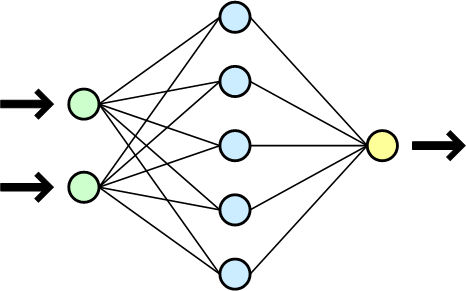
\includegraphics[width=250px]{Figures/Neuralnetwork.png}
\caption{Невронна мрежа}
\label{fig:NeuralNetwork}
\end{figure}

В невронната мрежа обикновено винаги съществуват входен и изходен слой от неврони, във входния се въвежда информацията към мрежата, след това сигналите от входните неврони преминават през един или няколко слоя от междинни (скрити) неврони, според топологията на невронната мрежа, като сигналите накрая стигат до изходния слой, откъдето се чете получената информация.

Теглата на връзките между невроните определят функционалността и поведението на невронната мрежа. За да бъде една невронна мрежа използваема и приложима към даден проблем, тя трябва да бъде предварително обучена.

Обучаването на една невронна мрежа се осъществавя с използване на тренировъчни данни, като в процеса на обучение се променят теглата на връзките между невроните търсейки се най-оптимални тегла спрямо тренировъчните данни. Най-разпространеното правило за това е метода на обратното разпространение на сигнал за грешка (back-propagation), където за всеки изходен неврон се изчислява разликата от желаното му поведение, като се формира сигнал за грешка, който се движи назад към входния слой и по пътя си променя теглата на връзките така, че при следващата активация на мрежата грешката да бъде по-малка от сегашната.

Невронните мрежи много се доближават до нашите мозъци по начина си на функциониране.  Изчисленията не се извършват на едно централно място, а са разпределени по цялата мрежа. Това прави мрежата изключително гъвкава, като тя продължава да работи дори когато от нея умишлено са премахнати изчислителни елементи. За сравнение, фон Ноймановата архитектура престава да функционира ако от нея липсва дори един елемент.

За съжаление, дори този модел на човешкия ум не е перфектен. Повечето съществуващи към момента изкуствени невронни мрежи не могат да моделират ефекта на хормоните върху мозъка. Освен това се оказва, че за да можем математически да опишем една изкуствена мрежа, в нея трябва да се спазват определени правила, например сигналите да се движат от входния към изходния слой, но не и обратно. (Съществуват и изкуствени мрежи, които са циклични, но поради повишената им сложност все още не са добре изучени.) Може би най-големият недостатък на невронните мрежи е, че тяхното обучение изисква множество повторения, а в много случаи човек научава дадена информация след като е бил изложен на нея само веднъж.

%----------------------------------------------------------------------------------------

\section{Задълбочено обучение (deep learning)}

Задълбоченото обучение е направление в машинното самообучение, който се основава на алгоритми, които целят да изградят абстракция от високо ниво на данните. Ако разгледаме един много прост случай може да имаме две множества неврони: едни, които получават входен сигнал и втори, които изпращат изходящ сигнал. Когато първият слой получи вход, той предава модифицирана версия на входа към следващия слой. При по-дълбока мрежа, има много слоя между входния и изходния, което позволява на алгоритъма за използва множество обработващи слоя, състоящи се от много трансформации. \cite{DeepLearningMethods} \cite{DeepArchitectures}

Дълбокото учение е част от по-голяма група методи в машинното самообучение, които се основават на обучение върху изгледа на данни. Наблюдение (например картинка) може да се представи по много начини като например вектор от интензивността на пикселите или по по-абстрактен начин като множество от ъгли, региони с определена форма и още много други. Някои изгледи са по-добри от други по отношение на опростяване на обучението. Една от основните дейности на задълбоченото обучение е, че се премахва нуждата от ръчно изваждане на модели от хора. На тяхно място се използват ефективни алгоритми за обучение и йерархично автоматично изграждане на модели.

Разработките в тази насока се стремят да се намерят тези модели в огромен обем необработени данни. Някои модели са вдъхновени от напредъка в неврологията и се основават на интерпретации на обработката на информация и начините на комуникация в нервната система.

Различни видове архитектури като Невронни мрежи, Конволюционни невронни мрежи, Deep belief мрежи и рекурентни невронни мрежи са прилагани в области като разпознаване на реч, обработка на естесвен език, разпознаване на звуци, биоинформатика, където те достигат най-точни резултати от всички използвани методи.

%----------------------------------------------------------------------------------------

\section{Конволюционни Невронни мрежи}

Този вид невронни мрежи за вдъхновени от визуалния кортекс при животните. Отделни неврони отговарят за стимулирането на ограничен район на действие, който се нарича област на възприемане. Когато полето на възприемане на даден неврон бъде задействано, неговият отговор може да бъде изчислен математически чрез конволюционна операция (convolutional). Вдъхновени са от биологични процеси и са вариация на многопластов перцептрон, който използва минимално количество предварителна обработка. Те са най-приложими в обработката на изображения и видеа, препоръчващите системи и обработката на естествен език. \cite{CNN_2} \cite{CNN_3}


\subsection{Област (поле) на възприемане}
През 50-те и 60-те години на 20 век труд на Хубел и Визел показва, че визуалния кортекс на котките и маймуните съдържа неврони, които индивидуално реагират на малки региони от визуалното поле. Регионът от визуалното поле, в който съдържанието въздейства на специфични неврони се нарича област (поле) на възприемане. Съседните клетки имат подобни и припокриващи се полета на възприемане. Размерът и мястото на областта на възприемане варира из корпуса, за да формира пълна карта на визуалното пространство. \cite{CNN_1}

\subsection{Специфични особености}
Въпреки, че стандартните невронни мрежи могат успешно да бъдат приложени за разпознаване на изображения, те имат сериозен недостатък при уголемяване на размерите на изображенията. Например при изображение с размери 32x32 пиксела и 3 цветови канала един пълно свързан неврон би имал 32*32*3=3072 тегла. При изображение с размери 500x500 броят им би бил 750 000. При наличието на следващ слой със същата големина броят на връзките би бил 562 500 000 000.
Освен това тази архитектура третира пиксели, които са раздалечени по един и същи начин като пиксели, които са един до друг. Очевидно пълната свързаност на невроните не е добро решение при задачата за разпознаване на изображения. Като следствие огромният брой параметри води до прекомерно нагаждане (overfitting). 
Конволюционните невронни мрежи имат следните специфични осоености
\begin{enumerate}
\item \textbf{3 измерения на невроните}. Слоевете имат неврони, организирани в 3 измерения: ширина, височина и дълбочина. Невроните във всеки слой са свързани само с малък брой от невроните в предишния слой (област на възприемане). Различни видове слоеве (както локално така и напълно свързани) се обединяват за да организират конволюционна невронна мрежа.
\item \textbf{Локална свързаност}: следвайки концепцията на полето на възприемане, този вид невронни мрежи използват локална свързаност като принуждават невроните от последователните слоеве да комуникират само с близките до тях съседи. По този начин архитектурата осигурява това, че научените "филтри" продуцират най-силна връзка при взаимодействие между близки неврони. Нареждането на много подобни връзки води до нелинейни филтри, които стават все по-глобални. Това позволява на мрежата първо да намери отличителни черти на малка част от входа и след това да види как те са приложени в по-голямо изображение.
\item \textbf{Споделени тегла}: Всеки филтър се прилага върху цялото визуално поле. Където се използват, тези единици споделят едни и същи тегла. Това означава, че всички неврони в даден слой засичат точно един и същи модел на свързаност. По този начин се позволява моделът да бъде намерен независимо къде се намира върху визуалното поле.
\end{enumerate}
Заедно тези свойства позволяват на конволюционните невронни мрежи да постигнат по-добра генерализация при визуалните проблеми. Споделянето на теглата драстично намалява броя на параметрите, които трябва да се обучат. По този начин се намаляват хардуерните изисквания за използване на невронната мрежа. Това от своя страна позволява тренирането на по-големи и по-мощни мрежи. 

\subsection{Видове слоеве}
Конволюционните невронни мрежи използват някои различни слоеве в сравнение със стандартните невронни мрежи. Такива са конволюционният слой, обединяващият слой и слоят на ректифицираните линейни единици (ReLU).

\ref{fig:ConvNeuralNetwork} показва примерна архитектура на конволюционна невронна мрежа.

\begin{figure}[H]
\centering
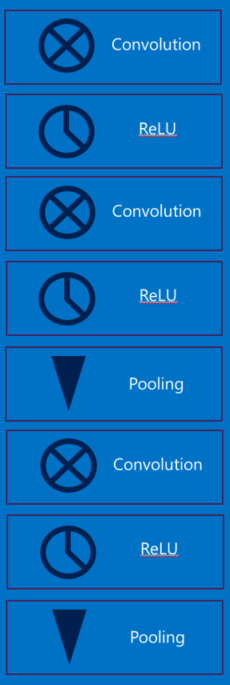
\includegraphics{Figures/cnn12.png}
\caption{Архитектура на конволюционна невронна мрежа \cite{CNN_blog}}
\label{fig:ConvNeuralNetwork}
\end{figure}

\subsubsection{Конволюционен слой}
Това е основата на този тип невронни мрежи. Параметрите на този слой са множество от самообучаващи се филтри, които имат малко поле на възприемане, но се разширяват до пълната дълбочина на входните параметри. При всяко предаване едно ниво напред всеки филтър създава своя карта в зависимост от това дали се среща или не по цялата ширина и височина на входа. Това означава, че се търси къде този филтър е наличен в подадения вход и се връща като резултат двуизмерна активационна карта, указваща местата на филтъра. Като резултат мрежата научава филтри, които се активират при специфичен модел на някоя позиция от входа.
Като се обединят активационните карти на всички филтри по измерението за дълбочина се оформя пълният изход от конволюционния слой. Всяка единица от изхода може да се интерпретира като резултат от неврон, който отговаря за малък регион от визуалното поле и споделя параметри с неврони от същата активационна карта.

Когато входните данни са от много високо измерение (както изображенията) не е практично да се свързват неврони с всички неврони от предходния слой, защото такава архитектура не взима предвид близостта на данните (например дали 2 пиксела са един до друг или раздалечени). Всеки неврон е свързан само с малък регион от входните данни. Големината на тези региони е хиперпараметър, който се нарича област на възприемане на неврона. Връзките са локални по отношение на ширина и височина, но винаги са по цялата дълбочина на входните данни. Такава архитектура гарантира, че научените филтри имат най-силно въздействие върху резултата.  

Три хиперпараметъра контролират размера на изхода на конволюционния слой: дълбочина, стъпка на алокиране и брой колони с добавени нули.
Дълбочината на изхода контролира броя неврони в слоя, които са свързани със същия регион от входния слой. Всички тези неврони ще се научат да се активират за различни модели на входа. Например, ако първият конволюционен слой приема необработено изображение като вход, различните неврони разположени в дълбочина може да се активират при наличие на различни ъгли, цветове или други форми. Стъпката (stride) се грижи за това как се оформят колоните в дълбочина около измеренията ширина и височина. Когато съпката е 1 се образува нова колона неврони, които са свързани само до единиците на разстояние 1. Това води до пренатоварване на полетата на възприемане между колоните и също така до огромни размери на изхода. Понякога е удобно да изместим входните данни като добавим нули на граничните стойности. Колко колони с нули ще добавим е третият хиперпараметър. Той ни дава контрол да определеми размера на изхода. 

В конволюционните слоеве се използва схема на споделяне на параметри  за контрол на броя на свободните параметри. То се основава на следното: ако даден модел е полезен в определен регион, то той би бил полезен дори да е намерен и на друга позиция. Тъй като всички неврони в един изрязък по отношение на дълбочина споделят един и същи параметри, изходът от всяка част от конволюционния слой може да се изчисли като конволюция от теглата на невроните към входните данни. Следователно, често срещано е да наричаме множество от тегла филтър (или ядро), който е свързан с вхдоните данни. Резултатът от конволюцията е активационна карта, и множеството такива карти за всеки филтър се напасват заедно по отношение на дълбочината за да генерират изходните данни. 
Важно е да се отбележи, че понякога споделянето на параметри може да не е подходящо. Такъв пример е когато входните изображения за невронната мрежа имат нещо специфично в центъра на изображенията и ние очакваме филтрите да бъдат намерени точно в централната част. Пример на практика е разпознаване на лица, където лицата са в центъра на изображението. В този случай избягваме споделянето на параметри и просто разчитаме на локално свързани слоеве.

\subsubsection{Обединяващ (Pooling) слой}
Друга важна концепция в конволюционните невронни мрежи е обединяването (pooling), което е вид нелинейно намаляване на пространство. Има няколко нелинейни функции, които имплементират обединяването. Най-популярната от тях е max pooling \ref{fig:MaxPooling}. При нея изображението се разделя на множество от непресичащи се правоъгълници и за всеки такъв регион връща максимума. Интиутивното обяснение е, че щом даден модел е бил намерен, неговото точно местоположение не е от толкова голямо значение колкото относителното му местоположение спрямо други модели. Основната роля на този слой е прогресивно да намали размера на данните в мрежата и следователно да се избегне прекомерното нагаждане. 
Този слой се изпълнява независимо за всяка дълбочина на входа и променя размерите независимо. Най-често срещаната форма в прилагане на pooling функция с филтри с размери 2x2 като по този начин се изоставят 75\% от активациите. По този начин всяка операция за максимизиране ще търси най-голямото от 4 числа. Измерението за дълбочина остава непроменено.
Други видове функции, които биха могли да бъдат приложени са средно аритметично намаляване и L2-нормализация. До скоро средно аритметичното намаляване е било предпочитано, но в последните години максимизирането дава по-добри резултати в практиката.

\begin{figure}[H]
\centering
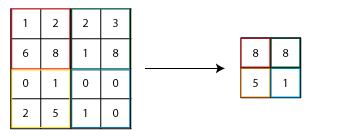
\includegraphics{Figures/Max_pooling.png}
\caption{Обединяващ (pooling) слой}
\label{fig:MaxPooling}
\end{figure}

\subsubsection{Слой на ректифицираните линейни единици (ReLU - Rectified Linear Units)}
Това е слой от неврони, който прилага активационната функция f(x)=max(0,x). Той повишава нелинейните свойства на функцията за взимане на решения и като цяло на мрежата без да оказва влияние на областите на възприемане на конволюционния слой.
Използват се и други функции за повишаване на нелинейността. Например f(x)=tanh(x) и f(x)=|tanh(x)|. ReLU е най-предпочитана в сравнение с другите функции, защото прави процеса на обучение на мрежата много по-кратък и няма големи разлики по отношение на точността.

\subsubsection{Напълно свързан слой}
Накрая след няколко конволюционни и обединяващи слоя взимането на решения се осъществява от напълно свързаните слоеве. Невроните в тях имат връзки със всички активации в предишния слой както при стандартните невронни мрежи. Тяхната активация би могла да се пресметне чрез матрица на умноженията, последвана от контролирано отклонение.

\subsubsection{Слой на наказанията}
Този слой указва как мрежата наказва разликата между предсказаните и истинските стойности и обикновено е последният слой в мрежата. Има различни функции за наказание в зависимост от конкретната задача. Softmax е една от тях и се използва, когато трябва да се предскаже 1 от няколко взаимно изключващи се класа. Това е и конкретният случай. Крос ентропичен сигмоид се използва при предсказване на K независими вероятности в диапазона [0,1].

\subsection{Избор на хиперпараметри}
\subsubsection{Брой филтри}
Тъй като с навлизане в невронната мрежа размерът на данните се намалява е удачно да имаме по-малко филтри в началото и повече в края. За да се уеднакви изчислителното време във всеки слой произведението на броя пиксели и броя модели е почти константно из всичките слоеве. За да се запази входната информация трябва да се осигури, че броят активации не трябва да намалява от един слой към следващия.

\subsubsection{Форма на филтрите}
Има много различни форми на филтрите и обикновено се избират в зависимост от входните данни.

\subsubsection{Максимални размери на формата за обединяване}
Обикновено обединяването се извършва върху 2x2 пиксела. При огромни входни данни може да бъде 4x4. Това обаче може да доведе до премахването на твърде много важна информация.

\subsection{Методи за регуларизация}

В сферата на машинното самообучение, под регуларизация се разбира процесът на добавяне на информация с цел да се реши проблемът с прекомерното нагаждане.

\subsubsection{Ранно прекратяване (Early stopping)}
Това е един от най-простите методи за предотвратяване на прекомерното нагаждане. Той предлага просто да прекратим тренирането преди нагаждането да може да се случи. Недостатъкът е, че обучението се прекратява преждевременно. Един от начините за прилагане на ранното прекратяване е да се следи грешката върху тренировъчното и валидационното множество и когато се види, че грешката върху валидационното спира да пада се спира обучението.


\subsubsection{Ограничаване на броя параметри}
Друг много прост подход е да се ограничат броят параметри в невронната мрежа. Обикновено се ограничава броят на скритите единици във всеки слой или дълбочината на невронната мрежа. За конволюционни невронни мрежи, размерът на филтрите също оказва влияние на броя на параметрите. Ограничаване на броя параметри намалява директно възможността на мрежата да предскаже резултат. Намалява се сложността на операциите, които се извършват върху данните и по този начин се намалява възможността за прекомерно нагаждане.

\subsubsection{Изкуствено добавяне на тренировъчни данни (Artificial data)}
Тъй като прекомерното нагаждане на модела се определя от неговата специфика и количеството тренировъчни данни, генерирането на допълнителни тренировъчни примери може значително да намали overfitting-а. Един от популярните подходи за генериране на нови примери е да се променят настоящите и да се подадат като нови примери. Например дадено изображение може да бъде завъртяно или изрязано на произволен принцип. Основна идея на този метод е моделът да не се преспецифицира към конкретното място, на което е показан обектът, но да е готов да го срещне и на друго място.

\subsubsection{Разпадане на теглото (Weight decay)}
При този подход ръчно добавяме допълнителна грешка към обучителните данни. Има различни начини за избиране на грешката - сума на всички тегла (L1 нормализация) или корен квадратен от сбора на квадратите на теглата (L2 нормализация). Може да се намали сложността на големи модели като се уголеми наложеното наказание върху векторите.

\subsubsection{Метод на отпадане (Dropout)}
Тъй като напълно свързаният слой има достъп до повечето параметри, той е податлив на прекомерно нагаждане (overfitting). Методът на отпадане е емпиричен и се грижи това да не се случи. На всяка итерация на трениране всяка нишка или отпада с вероятност 1-p или остава с вероятност p. По този начин остава редуцирана мрежа като входящите и изходящите нишки също се премахват. След това само редуцираната мрежа се тренира. След това премахнатите елементи се добавят на ново в мрежата с първоначалните им тегла.
По време на етапите на трениране, вероятността даден елемент да се запази е обикновено 0.5. За входящи нишки вероятността трябва да е много по-висока, защото информацията просто изчезва, когато игнорираме входящи данни.
Като не тренираме върху всички връзки от тренировъчните данни, методът на отпадане намалява прекомерното нагаждане в невронните мрежи. Освен това той значително подобрява времето за трениране. Това прави комбинациите на модела подходящи дори за много дълбоки невронни мрежи. Тази техника намалява сложността на взаимодействието между слоевете и спомага за научаването на по-генерални модели. Използва се за подобряване на продуктивността на невронни мрежи при задачи като визуално и гласово разпознаване, класификация на документи и биологични проблеми.

\subsubsection{Метод на премахване на връзките (DropConnect)}
Този метод е генерализация на Dropout, при която всяка връзка (вместо всяка изходяща единица) може да отпадне с вероятност 1-p. По този начин всеки неврон получава данни от произволни единици от предишния слой.
Този метод е много подобен на Dropout, защото позволява динамично разреждане на модела, но се различава по това, че премахването на данни е от теглата, а не от изходящите вектори на слоя. С други думи, при този подход напълно свързаният слой става частично свързан, като връзките, които остават са избрани на произволен принцип.

\subsubsection{Стохастично обединяване (Stochastic pooling)}
При стохастичното обединяване се оформят региони на действие. За всеки регион се избира активация според полиномиално разпределение, което е следствие от действията в този регион. Този подход не зависи от външни параметри и може да бъде комбиниран с други методи за регуларизация. 
Друг начин на представяне на този метод е, че той е същият като максимално обединение (max pooling), но върху много копия на едно и също изображение, като всяко от копията има малки локални промени. Методът е подобен на предварителна обработка на входните изображения, което води до много добро представяне в някои случаи. Използването на метода при архитектура с многослоен модел води до експоненциален брой деформации, защото промените в началните слоеве са независими от тези в последващите.

\section{Състезанието на ImageNet}

\subsection{Въведение}

Състезанието на ImageNet Large Scale Visual Recognition Challenge (ILSVRC) \cite{ILSVRC15} оценява алгоритми за разпознаване на обекти и класифициране на изображения в огромни мащаби. Една от основните цели е да позволи на изследователите в тази област да сравнят постигнатите от тях резултати при наличието на голямо разнообразие от данни, възползвайки се от ръчно обработени картинки. Друга полза е да се види докъде е стигнал глобалният прогрес по разпознаване на изображения и автоматичната им анотация.

Състезанието е ежегодно и в него се включват най-големите компании в областта. За всяко издание се организира конференция, на която се споделят най-добрите методи и резултатите от текущото издание.

\subsection{Подробен преглед на победителя в ILSVRC 2015}
Победителите са от Microsoft Research Asia (MSRA). Те предоставят две архитектури: директна (plain) и остатъчна (residual) \cite{He2015}. При директната конволюционните слоеве имат филтри с размери 3x3 и следват 2 основни правила:
\begin{enumerate}
\item За даден размер на изхода, слоевете имат същия брой филтри.
\item Aко размерът на функция на картата е намалена наполовина, броят на филтрите се удвоява, така че да се запази сложността.
\end{enumerate}
Стъпката (stride) е 2. Мрежата свършва с напълно свързан слой с 1000 неврона и softmax активационна функция. Общият брой слоеве са 34.
Остатъчната мрежа е базирана на първата като се добавят кратки пътища \ref{fig:plain_residual}.

Те могат да се използват, когато входът и изходът са с едни и същи размери. Когато са с различни размери има два подхода:
\begin{enumerate}
\item Добавят се нули, за да се уеднакви размерът.
\item Използва се проекция, за да се уеднакви размерът.
\end{enumerate}

Авторите сравняват мрежи с различен брой слоеве, като на \ref{fig:plain_residual_charts} са показани резултатите при 16 и 34 слоя за стандартни и остатъчни мрежи:

\begin{figure}[H]
\centering
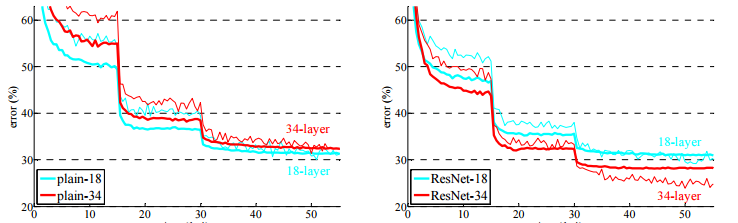
\includegraphics[width=400pt]{Figures/plain_residual_charts.PNG}
\caption{Графики на резултатите при 16 и 34 слоя за стандартни и остатъчни мрежи \cite{He2015} }
\label{fig:plain_residual_charts}
\end{figure}

\begin{figure}[H]
\centering
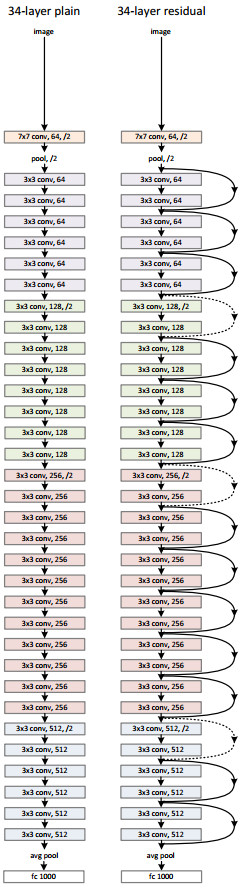
\includegraphics[height=620pt]{Figures/plain_residual.PNG}
\caption{Сравнение на архитектурата на стандартна и остатъчна мрежа \cite{He2015} }
\label{fig:plain_residual}
\end{figure}

Първоначално изображенията се намаляват до размери [256, 480], след което се взима произволен участък с размери [224, 224]. За класификационната задача тестовете са извършени върху 1000 класа с 1 280 000 тренировъчни изображения и 50 000 тестови.

Изпробвани са остатъчни невронни мрежи с 16, 34, 50, 101 и 152 слоя. Има и 2 вида мерки за точност: при първия (top 1) се връща само 1 клас и точността е процентът изображения, за които правилният клас е избран. При втория (top 5) един опит се счита за успешен ако търсеният клас е един от първите 5 върнати класа от невронната мрежа. Най-добрите постигнати резултати са с мрежа със 152 слоя (19.38\% и 4.49\% грешка съответно за top 1 и top 5) \ref{tab:table_results_architectures}.

\begin{longtable}{ | c | c | c | }
\hline
\textbf{Модел} & \textbf{top 1 грешка} & \textbf{top 5 грешка} \\ \hline \hline
ResNet-34 B & 21.84 & 5.71 \\ \hline
ResNet-34 C & 21.53 & 5.60 \\ \hline
ResNet-50   & 20.74 & 5.25 \\ \hline
ResNet-101  & 19.87 & 4.60 \\ \hline
ResNet-152  & \textbf{19.38} & \textbf{4.49} \\ \hline
\caption{Резултати при различните архитектури на невронни мрежи \cite{He2015} }
\label{tab:table_results_architectures}
\end{longtable}
 
\chapter{Използвани технологии и платформи}

\label{Chapter3}

%----------------------------------------------------------------------------------------

\section{Обучителни данни}

ImageNet е огромна база от данни с изображения, предназначена за използване от разработчици на софтуери за разпознаване на изображения. От 2016 година, повече от 10 милиона изображения са анотирани ръчно от ImageNet, за да покажат какви обекти са показани. Очертаващи линии на обектите в изображенията са дадени за над 1 милион картинки \cite{ImageNet}. Базата с изображения, както и техните анотации е свободно достъпна в ImageNet, но те не са тяхно притежание.

Процесът на анотация се извършва чрез външни хора. Анотациите на ниво изображение индикират наличието или липсата на даден клас в картинката. Анотациите, които са за конкретен обект от картинката предоставят и ограждащи граници на обекта (видимата му част върху изображението). ImageNet използва йерархична словесна схема за организация като поддържа клас куче и над 120 под-класа, които са различни породи кучета. Това позволява избор на разработчиците колко прецизно и на какво ниво на абстракция искат да е класифицирането.

С цел обучение бяха изтеглени 57 класа животни, съдържащи между 1500 и 2000 изображения за клас. Те са с различни размери и обхващат разнообразни фонове и среди. Изтеглените класове са показани на Фигура \ref{tab:tableclasses}.

\begin{longtable}{ | c | c | c | }
\hline
\textbf{Номер} & \textbf{Име} & \textbf{Идентификатор} \\ \hline \hline
0 & alligator & n01698434 \\ \hline
1 & antelope & n02419796 \\ \hline
2 & bat & n02139199 \\ \hline
3 & bear & n02131653 \\ \hline
4 & bison & n02410509 \\ \hline
5 & butterfly & n02274259 \\ \hline
6 & camel & n02437136 \\ \hline
7 & canary & n01533339 \\ \hline
8 & cat & n02121808 \\ \hline
9 & cattle & n04052442 \\ \hline
10 & chicken & n01791625 \\ \hline
11 & cockroach & n02233338 \\ \hline
12 & deer & n02430045 \\ \hline
13 & dog & n02084071 \\ \hline
14 & donkey & n02389559 \\ \hline
15 & duck & n01846331 \\ \hline
16 & eagle & n01613294 \\ \hline
17 & elephant & n02503517 \\ \hline
18 & fly & n02190166 \\ \hline
19 & fox & n02118333 \\ \hline
20 & frog & n01641739 \\ \hline
21 & giraffe & n02439033 \\ \hline
22 & goat & n02416880 \\ \hline
23 & goldfish & n01443537 \\ \hline
24 & horse & n02374451 \\ \hline
25 & hyena & n02116738 \\ \hline
26 & iguana & n01677366 \\ \hline
27 & jaguar & n02128925 \\ \hline
28 & kangaroo & n01877134 \\ \hline
29 & lion & n02129165 \\ \hline
30 & llama & n02437616 \\ \hline
31 & monkey & n02484322 \\ \hline
32 & mosquito & n02200198 \\ \hline
33 & mouse & n02330245 \\ \hline
34 & octopus & n01970164 \\ \hline
35 & ostrich & n01518878 \\ \hline
36 & owl & n01621127 \\ \hline
37 & panda & n02510455 \\ \hline
38 & parrot & n01817346 \\ \hline
39 & penguin & n02055803 \\ \hline
40 & pig & n02395406 \\ \hline
41 & pigeon & n01814921 \\ \hline
42 & piranha & n02584449 \\ \hline
43 & rabbit & n02324587 \\ \hline
44 & raven & n01579260 \\ \hline
45 & scorpion & n01770393 \\ \hline
46 & shark & n01482330 \\ \hline
47 & sheep & n10588074 \\ \hline
48 & snail & n01944390 \\ \hline
49 & snake & n01726692 \\ \hline
50 & spider & n01772222 \\ \hline
51 & swan & n01858441 \\ \hline
52 & tiger & n02129604 \\ \hline
53 & turkey & n01794344 \\ \hline
54 & whale & n02062744 \\ \hline
55 & worm & n01922303 \\ \hline
56 & zebra & n02391049 \\ \hline
\caption{Обучително множество от класове}
\label{tab:tableclasses}
\end{longtable}

\section{Технологии, платформи и методологии}
Една от основните причини разпознаването на изображение да бъде възможно е напредъкът на хардуера и възможността да използваме мощността и бързия достъп до паметта на видео картите (GPU). Един от най-удобните начини това да се случи се предоставя от CUDA \cite{CUDA}. Като програмен език е избран Python \cite{Python}, който е най-популярното решение в тази сфера, защото предоставя лесна интеграция с интерфейси за достъп до видео картата и има много популярни и добри библиотеки за изкуствен интелект. За изграждане на конволюционните невронни мрежи се използва TensorFlow \cite{Tensorflow}. За управление на версиите се разчита на скрито Git хранилище в Bitbucket \cite{Bitbucket}.

\subsection{CUDA}
CUDA е платформа за паралелна обработка и програмен интерфейс (API), създаден от Nvidia. Той позволява на софтуерните разработчици да използват видео карти, които позволяват CUDA за обработка с каквато и да е цел - този подход се нарича GPGPU (General-Purpose computing on Graphics Processing Units). CUDA платформата е софтуерен слой, който позволява директен достъп до видео картата и елементите за паралелна обработка за всякакви изчислителни цели. \cite{EndOfCPU}

CUDA е предназначен за работа с програмни езици като C,C++ и Фортран. Тази достъпност прави по-лесен за специалистите по паралелна обработка да използват ресурсите на видео картата за разлика от други услуги като Direct3D и OpenGL, които изискват добри умения в графичното програмиране. Също така CUDA поддържа програмни среди като OpenACC и OpenCL. Когато за първи път е представен от Nvidia, CUDA е бил абревиатура на Compute Unified Device Architecture, но впоследствие Nvidia се отказва от съкращението.

CUDA предоставя услуги както на ниско, така и на високо ниво на абстракция. Първата услуга CUDA пуска в публичното пространство на 15.02.2007г. с поддръжка на Windows и Linux. Mac OS X поддръжка се добавя във версия 2.0. CUDA работи с всички видео карти на Nvidia и повечето стандартни операционни системи.

\subsection{Python}

Python е глобално използван динамичен език за програмиране от високо ниво \cite{Python_1}. Философията на неговия дизайн набляга на четимост на кода и неговият синтаксис позволява на програмистите да имплементират концепции с по-малко линии код в сравнение с други езици като C++ и Java. Езикът предоставя конструкции, които са предназначени за писане на чист код както за малки, така и за големи програми. \cite{Python_2}

Python поддържа множество програмни парадигми като обектно-ориентирано, императивно, функционално програмиране и процедурни стилове. При него има динамично типизиране и автоматично управление на паметта. Има много и качествени налични библиотеки.

Python интерпретатори са налични за много операционни системи, което позволява да се изпълнява Python код при почти всякакви системи. CPython, както и повечето различни имплементации на Python са с отворен код.

\subsubsection{Структура и функционалност}
Python предлага добра структура и поддръжка за разработка на големи приложения. Той притежава вградени сложни типове данни като гъвкави масиви и речници, за които биха били необходими дни, за да се напишат ефикасно на C.

Python позволява разделянето на една програма на модули, които могат да се използват отново в други програми. Също така притежава голям набор от стандартни модули, които да се използват като основа на програмите. Съществуват и вградени модули, които обезпечават такива неща като файлов вход/изход (I/O), различни системни функции, сокети (sockets), програмни интерфейси към GUI-библиотеки като Тк, както и много други.

Тъй като Python е език, който се интерпретира, се спестява значително време за разработка, тъй като не са необходими компилиране и свързване (linking) за тестването на дадено приложение. Освен това, бидейки интерпретируем език с идеология сходна с тази на Java, приложение, написано на него, е сравнително лесно преносимо на множеството от останали платформи (или операционни системи).

Програмите, написани на Python, са доста компактни и четими, като често те са и по-кратки от еквивалентните им, написани на C/C++. Това е така, тъй като:

\begin{itemize}
\item наличните сложни типове данни позволяват изразяването на сложни действия с един-единствен оператор;
\item групирането на изразите се извършва чрез отстъп, вместо чрез начални и крайни скоби или някакви други ключови думи (друг език, използващ такъв начин на подредба, е Haskell);
\item не са необходими декларации на променливи или аргументи.
\item Python съдържа прости конструкции, характерни за функционалния стил на програмиране, които му придават допълнителна гъвкавост
\end{itemize}

Всеки модул на Python се компилира преди изпълнение до код за съответната виртуална машина. Този код се записва за повторна употреба като .pyc файл.

Програмите написани на Python представляват съвкупност от файлове с изходен код. При първото си изпълнение този код се компилира до байткод, а при всяко следващо се използва кеширана версия. Байткодът се изпълнява от интерпретатор на Python.

\begin{itemize}
\item Строго типизиран (strong typing) – При несъответствие между типовете е необходимо изрично конвертиране.
\item Динамично типизиран (dynamic typing) – Типовете на данните се определят по време на изпълнението. Работи на принципа duck typing – Оценява типа на обектите според техните свойства.
\item Използва garbage collector – вътрешната реализация на езика се грижи за управлението на паметта.
\item Блоковете се формират посредством отстъп. Като разграничител между програмните фрагменти използва нов ред.
\end{itemize}

\subsection{Tensorflow}

Tensorflow e софтуерна библиотека с отворен код за числови изчисления с помощта на графи за предаване на данните (data flow graphs). Всеки връх в графа представлява математически операции, докато пътищата са многомерни масиви (тенсори - tensors), които служат за комуникация между тях. Архитектурата позволява да се извършват изчисления на повече от един процесор или видео карта както на десктоп, така и на сървър или мобилно устройство използвайки един единствен програмен интерфейс (API). Tensorflow първоначално е разработен от изследователи и инженери, работещи в Google по проекта Google Brain \cite{GoogleBrain} по разработка за изследователската организация Google's Machine Intelligence. Първоначалната им цел е била изследване в сферите на машинното самообучение и невронните мрежи, но системата е достатъчно генерална, за да се прилага свободно и в други области. \cite{Tensorflow}

\subsubsection{Въведение}

Проектът Google Brain стартира през 2011, за да изследва използването на дълбоки невронни мрежи с много големи мащаби както с изследователска цел така и за да се използва от Google. Като част от началната работа по този проект първо е построен DistBelief, система от първа генерация за скалируемо трениране. Благодарение на DistBelief са извършени множество изследователски дейности като обучение без надзор, репрецентация на езици, модели за класифициране на изображения, разпознаване на обекти, класификация на видеа, разпознаване на реч, игра на Go, разпознаване на граждани и множество други сфери \cite{TensorflowDetails}. Освен това често след взаимодействие с екипът Google Brain, повече от 50 други екипи от Google и други комнпании са използвали дълбоки невронни мрежи с помощта на DistBelief в много продукти, сред които Google Search, рекламни продукти, системи за разпознаване на реч, Google Photos, Google Maps и StreetView, Google Translate, YouTube и много други. 

На база на опита, придобит от DistBelief и след по-добро разбиране на това какво е нужно да има такава система е създаден Tensorflow - система от втора генерация за имплементиране и използване на модели за машинно самообучение от големи мащаби. Tensorflow чете изчисленията с модел, който използва поток от данни и ги нагажда спрямо голямо разнообразие от хардуерни платформи. Той може да се използва както от мобилни устройства с Android или iOS, така и от отделни машини с една или повече видео карти. Налична е поддръжката и на паралелна работа върху много машини. Разполагайки с една система, която може да се изпълнява върху голям набор от хардуерни платформи значително опростява използването на системи за машинно самообучение. Изчисленията в Tensorflow са представени като графи на данните със състояния. Той позволява бързи експерименти с нови модели за изследователски цели и предоставя много висока производителност. С цел да се скалира тренирането на невронни мрежи за по-големи системи, Tensorflow позволява лесно да се изградят паралелни операции на различни машини, които обновяват множество споделени параметри и състояния. Лесният за употреба интерфейс позволява да се постигат различни техники за паралелна обработка с много малко усилия. Някои употреби на Tensorflow позволяват гъвкавост по отношение на цялостност при обновяването на параметрите и това много лесно може да се използва при големи системи. В сравнение с DistBelief, програмният модел на Tensorflow е по-гъвкав, неговата производителност е значително по-добра и поддържа използване на по-голямо множество от модели върху повече хардуерни платформи.

\subsubsection{Програмен модел и основни концепции}

Изчисленията в Tensorflow представляват насочен граф, който е изграден от множество върхове. Графът представлява изчисление на поток от данни с разширения, които позволяват някои пътища да не се променят и дават контрол вътху разклоненията и циклите на пътищата в графа. Най-честите употреби на Tensorflow са чрез езиците за програмиране C++ и Python.

В графа на TensorFlow всеки връх има 0 или повече входа и 0 или повече изхода и представлява инстанция на една операция. Стойности, които се пренасят по стандартните пътища в графа се наричат тензори. Те са масиви с променливи измерения, при които типът на данните се определя при създаване на графа. Има и специални пътища, които контролират зависимостите. През тях не се предават данни, но те синхронизират работата на останалите пътища и определят кога дадена операция да започне да се изпълнява. Tensorflow понякога автоматично добавя такива специални пътища, за да въведе ред над независими до преди този момент операции. Това се прави с различни цели като например оптимизирано използване на паметта.\\

\textbf{Операции и ядра}

Всяка операция има име и представлява абстракция на изчисление (например умножение на матрици или събиране). Операциите могат да имат атрибути и всички атрибути трябва да бъдат дефинирани по време на изграждане на графа, за да се създаде връх в него, който да отговаря за операцията. Една от честите употреби на атрибутите е една операция да се направи полиморфна върху различни типове данни.

Под ядро се разбира конкретна имплементация на операция, която може да се изпълни върху конкретен вид устройство (например процесор или видео карта). Tensorflow дефинира видовете операции и ядра посредством механизъм за регистрация. Това множество може да се разширява чрез свързване на допълнителни дефиниции на операции и/или ядра.\\

\textbf{Сесии}

Всяка клиентска програма взаимодейства със системата на Tensorflow като създава нова сесия. С цел да създаде граф на изчисленията, интерфейсът на сесията поддържа метод за разширение, за да разшири графа с допълнителни върхове и пътища (при създаване на сесията графът е празен). Другата основна операция, която се поддържа от интерфейса на сесията е "Стартирай" (Run), която приема множество изходи, които трябва да се изчислят, както и множество тензори, които могат да се добавят към графа. В повечето случаи на употреба на Tensorflow след като веднъж се създаде сесия с граф, върху нея се извършват хиляди или милиони стартирания.\\

\textbf{Операция Variable}

При повечето изчисления един граф се използва много пъти. Повечето тензори не оцеляват по време на едно изпълнение на графа. Variable обаче е специален вид операция, която генерира връзка към постоянен непроменящ се тензор, който се запазва след няколко изпълнения върху графа. Тези връзки мгоат да бъдат предадени към специални операции като Assign или AssignAdd, които изменят съответния тензор. За приложенията на Tensorflow, свързани с машинно самообучение, параметрите на модела обикновено се пазят в тензори, които се пазят в променливи (Variable) и се обновяват, когато се стартира тренировъчния граф за модела.\\

\textbf{Алтернативи}

Theano също е библиотека в Python за цифрови изчисления. При нея те са представени с помощта на Numpy синтаксис \cite{Theano} и могат да се използват както върху процесор, така и върху видео карта. Theano е с отворен код и е основно разработен от група за машинно самообучение от Университета на Монреал.

Caffe е библиотека, написана на C++. Първо е започната като докторантски проект в UC Berkeley, след което става с отворен код и за развитието ѝ допринасят много програмисти.

Има и други алтернативи на Tensorflow като Torch, CNTK (Computational Network Toolkit) на Microsoft, DSSTNE (Deep Scalable Sparse Tensor Network Engine) на Amazon.

\subsection{Keras}

Keras е библиотека за невронни мрежи от високо ниво. Написана е на Python и може да използва Tensorflow или Theano. Първоначалната ѝ цел е била да позволи бързи и лесни експерименти. Философията на създателите е, че възможността да стигнеш от идея до резултат за възможно най-кратко време е ключът към успешните изследователски дейности.

Сред основните предимства на библиотеката са:
\begin{itemize}
\item Модулярност: Слоевете на невронната мрежа, оптимизаторите, активационните функции, схемите за регуларизация са независими модули, които могат да се комбинират, за да създадат нов модул.
\item Опростена имплементация: Всеки модул е кратък и лесен за разбиране. Всеки ред код е интуитивен за четене още при първия преглед на имплементацията.
\item Възможност за разширяване: Много е лесно да се добавят нови модули, а за вече съществуващите са предоставени множество примери. Това прави Keras подходящ и за по-сложни изследователски цели.
\item Директна работа с Python. Няма нужда да се добавят допълнителни модули или конфигурационни файлове.
\end{itemize}

\subsection{Git}

Git е система за управление на версиите, следене на промените на компютърни файлове и координиране на работата по тези файлове с други хора. Той основно се използва за софтуерна разработка, но може да се използва и за други цели. Основните му приоритети са скорост, интегритет на данните и поддръжка на дистрибутирани, нелинейни процеси.

Git е създаден от Линус Торвалдс през 2005 година, за да се разработи ядрото на Линукс заедно с други разработчици, които допринасят за първоначалния му напредък.

Както и повечето други системи за управление на версиите (и за разлика от повечето системи с начин на комуникация клиент-сървър), всяка Git директория на всеки компютър съдържа в себе си цялата информация и история за хранилището. Това позволява пълно следене на версиите, независимо от наличието на мрежа или централен сървър.


\chapter{Реализация, експерименти и анализ на резултатите}

\label{Chapter4}

%----------------------------------------------------------------------------------------

\section{Реализация}

Системата за класификация на изображения е разработена на Python, използвайки PyCharm \cite{Pycharm}. \ref{fig:ProcessFlow} показва процеса на работа на системата.

\begin{figure}[H]
\centering
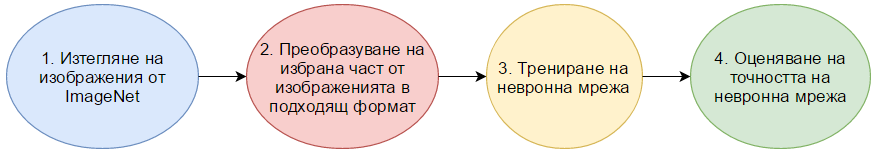
\includegraphics[width=400px]{Figures/ProcessFlow.PNG}
\caption{Начин на работа на системата}
\label{fig:ProcessFlow}
\end{figure}

\subsection{Събиране на данни и подготовка за обработка}

Подготвени са 57 класа животни, показани в \ref{tab:tableclasses}. \textbf{imagenet\_metadata.py} съдържа информация за тях във формат:

\begin{center}
<индекс, наименование, идентификатор в ImageNet>
\end{center}

\textbf{image\_crawler.py} изтегля всички снимки от извадените класове в директория, която е релативно разположена до основната. Създава се папка \_DATA, в нея папка ImageNet и в нея по една папка за всеки клас изображения. В нея съответно са изображенията.

Файлът \textbf{bin\_generator.py} създава файлове с разширение .bin, които представляват изображенията в удобен за четене формат. От картинките се взимат толкова класа, колкото е посочено в конфигурацията. Преди да се запишат картинките се преоразмеряват отново в зависимост от конфигурацията. За тестовете, извършени на локална машина, картинките се представят в размер 64x64 пиксела.

\subsection{Трениране и оценка на конволюционни невронни мрежи}

Файловете в директорията main отговарят за тренирането и оценка на невронни мрежи върху изтеглените и обработени изображения. \textbf{common.py} съдържа общи за системата функционалности. В \textbf{models.py} са дефинирани използваните архитектури. \textbf{train.py} зарежда избраната невронна мрежа и посочени от потребителя класове изображения и тренира върху тях. След това тя запазва модела, за да може да се преизползва в папката на генерираните .bin файлове. \textbf{eval.py} използва този модел и дава подробна оценка за точността разпределена по обучаваните класове. Имплементирана е крос валидация, която помага за по-точната оценка на моделите. \textbf{retrain.py} взима съществуващ модел, налага промени върху него (замразява слоеве, добавя нови, премахва ги) и продължава тренирането на избраната мрежа.

\subsection{Конфигурация и основни дефиниции}

Стартовата точка на системата е \textbf{main.py}. Нейната единствена роля е да предостави избор на потребителя какво иска да направи в текущата итерация на програмата. Предоставят се 4 възможности:
\begin{enumerate}
\item Изтегляне на данни
\item Превръщане на изображенията в подходящ за четене от програмата формат
\item Трениране на конволюционна невронна мрежа
\item Оценяване на вече трениран модел на конволюционна невронна мрежа
\end{enumerate}

За всички пътища в системата се грижи \textbf{definitions.py}. Той е в основната директория на програмата и съдържа всички нужни пътища в системата като например къде да се запазят изтеглените изображения, къде да се запазят натренираните модели и други.

Всички конфигуриации на системата се контролират от \textbf{src/config.py}. Параметрите, които подлежат на конфигурация са следните:

\begin{enumerate}
\item \textbf{IMAGE\_SIZE}: Размер на изображението в пиксели след обработка
\item \textbf{NUM\_CLASSES}: Брой класове, върху които да се тренира невронната мрежа
\item \textbf{EPOCHS}: Брой итерации, които се извършват при трениране на невронна мрежа
\item Други конфигурации на невронната мрежа
\item \textbf{CROSS\_VALIDATION\_ENABLED}: Флаг, указващ дали крос валидацията е позволена
\item \textbf{N\_FOLD\_CROSS\_VALIDATION}: На колко части да се разделят данните при използване на крос валидация
\item Имена на файлове, използвани в системата
\item Брой и размер на филтрите в конволюционните невронни мрежи
\end{enumerate}

\subsection{Тестове върху програмния код на победителя в победителя в ILSVRC 2015}
Директорията \textbf{pretrained} съдържа кода на едно от най-добрите решения до момента в областта \cite{He2015}. Той е публичен \cite{PretrainedGithub} и предоставя функционалности за класифициране на изображения, търсене на отличителни черти (features) в изображения и изкарване на отличителни черти от междинен слой на невронната мрежа. В \textbf{test\_imagenet.py} са имплементирани тестове върху готовите модели.

\section{Направени експерименти}

\subsection{Избор на архитектура}

Извършените опити за трениране на невронна мрежа се основават на 3 архитектури и техни разновидности с добавката на няколко параметъра. Първата е базова архитектура на конволюционна невронна мрежа, а другите 2 са на база на опити върху други данни с изображения CIFAR10 \cite{KerasTutorial}. Техните разновидности са направени с цел подобряване на резултатите и избягване на прекомерното нагаждане.

Архитектура 0 (\ref{tab:Architecture0}) е базова и съдържа само основни слоеве. 

\begin{longtable}{ | c | c | }
\hline
\textbf{№} & \begin{tabular}{@{}c@{}}\textbf{Архитектура 0} \\ (8 слоя)\end{tabular} \\ \hline \hline
1 & Конволюционен \\ \hline
2 & Max pooling \\ \hline
3 & Конволюционен \\ \hline
4 & Max pooling \\ \hline
5 & \begin{tabular}{@{}c@{}}Преминаване към \\ 1 измерение\end{tabular} \\ \hline
6 & \begin{tabular}{@{}c@{}}Напълно свързан \\ (softmax активация)\end{tabular} \\ \hline
\caption{Архитектура 0 на конволюционни невронни мрежи и нейните разновидности}
\label{tab:Architecture0}
\end{longtable}

\ref{plot:plt_arch0} показва резултатите при базовата Архитектура 0. Върху тестовите данни се забелязва растеж само до 7-8 итерация.

\begin{figure}[H]
\centering
\begin{tikzpicture}
\begin{axis}[]
\addplot[
    color=blue,
    mark=square,
    ]
    coordinates {
    (1, 33.28)
    (2, 44.72)
    (3, 48.91)
    (4, 52.50)
    (5, 55.59)
    (6, 56.59)
    (7, 59.35)
    (8, 61.58)
    (9, 64.37)
    (10,65.68)
    (11,65.39)
    (12,67.74)
    (13,68.77)
    (14,71.51)
    (15,72.72)
    (16,73.65)
    (17,76.31)
    (18,77.50)
    (19,79.09)
    (20,80.49)
    (21,81.25)
    (22,83.35)
    (23,84.58)
    (24,85.52)
    (25,87.47)
    };
\addplot[
    color=red,
    mark=*
    ]
    coordinates {
    (1, 41.66)
    (2, 47.17)
    (3, 49.72)
    (4, 53.45)
    (5, 53.59)
    (6, 56.28)
    (7, 55.17)
    (8, 58.00)
    (9, 59.10)
    (10,58.41)
    (11,59.38)
    (12,59.52)
    (13,57.66)
    (14,59.45)
    (15,59.31)
    (16,59.52)
    (17,59.52)
    (18,60.83)
    (19,61.17)
    (20,60.69)
    (21,59.38)
    (22,59.52)
    (23,60.97)
    (24,59.79)
    (25,61.52)
    };
\legend{Точност за тренировъчните данни,Точност за тестовите данни}
\end{axis}
\end{tikzpicture}
\caption{Точност на \textbf{Архитектура 0} при \textbf{5 класа}}
\label{plot:plt_arch0}
\end{figure}

Архитектура 1 (\ref{tab:Architecture1}) е кратка и се състои от 8 слоя. Нейната разновидност 1.1 добавя 2 слоя: напълно свързан и слой на отпадане основно с цел да да се избегне прекомерното нагаждане.

\begin{longtable}{ | c | c | c | }
\hline
\textbf{№} & \begin{tabular}{@{}c@{}}\textbf{Архитектура 1} \\ (8 слоя)\end{tabular} & \begin{tabular}{@{}c@{}}\textbf{Архитектура 1.1} \\ (10 слоя)\end{tabular} \\ \hline \hline
1 & Конволюционен & Конволюционен \\ \hline
2 & Dropout 0.2 & Dropout 0.2 \\ \hline
3 & Конволюционен & Конволюционен \\ \hline
4 & Max pooling & Max pooling \\ \hline
5 & \begin{tabular}{@{}c@{}}Преминаване към \\ 1 измерение\end{tabular} & \begin{tabular}{@{}c@{}}Преминаване към \\ 1 измерение\end{tabular} \\ \hline
6 & \begin{tabular}{@{}c@{}}Напълно свързан \\ (512 неврона)\end{tabular} & \begin{tabular}{@{}c@{}}Напълно свързан \\ (512 неврона)\end{tabular} \\ \hline
7 & Dropout 0.5 & Dropout 0.5 \\ \hline
8 & \begin{tabular}{@{}c@{}}Напълно свързан \\ (softmax активация)\end{tabular} & \begin{tabular}{@{}c@{}}\textbf{Напълно свързан} \\ \textbf{(256 неврона)}\end{tabular} \\ \hline
9 & - & \textbf{Dropout 0.3} \\ \hline
10 & - & \begin{tabular}{@{}c@{}}Напълно свързан \\ (softmax активация)\end{tabular} \\ \hline
\caption{Архитектура 1 на конволюционни невронни мрежи и нейните разновидности}
\label{tab:Architecture1}
\end{longtable}

\ref{plot:plt_arch1} показва резултатите при Архитектура 1. Значителен растеж се наблюдава до десетата итерация на трениране. След това спира растежа върху тестовите данни и значитено нараства този при тренировъчните. Финалните резултати са 96.89\% точност за тренировъчните и 62.41\% за тестовите.

\begin{figure}[H]
\centering
\begin{tikzpicture}
\begin{axis}[]
\addplot[
    color=blue,
    mark=square,
    ]
    coordinates {
    (1,33.23)
    (2,43.24)
    (3,46.10)
    (4,49.71)
    (5,52.38)
    (6,53.80)
    (7,56.63)
    (8,59.44)
    (9,61.37)
    (10,65.10)
    (11,66.72)
    (12,71.12)
    (13,75.02)
    (14,77.00)
    (15,81.76)
    (16,84.49)
    (17,86.63)
    (18,89.51)
    (19,90.77)
    (20,93.13)
    (21,95.20)
    (22,95.36)
    (23,96.57)
    (24,96.79)
    (25,96.89)
    };
\addplot[
    color=red,
    mark=*
    ]
    coordinates {
    (1,42.69)
    (2,45.10)
    (3,49.10)
    (4,52.34)
    (5,51.24)
    (6,55.10)
    (7,56.07)
    (8,58.21)
    (9,57.52)
    (10,57.45)
    (11,58.34)
    (12,60.41)
    (13,60.62)
    (14,59.03)
    (15,61.66)
    (16,60.90)
    (17,60.55)
    (18,60.21)
    (19,60.83)
    (20,61.03)
    (21,60.83)
    (22,61.31)
    (23,61.24)
    (24,62.14)
    (25,62.41)
    };
\legend{Точност за тренировъчните данни,Точност за тестовите данни}
\end{axis}
\end{tikzpicture}
\caption{Точност на \textbf{Архитектура 1} при \textbf{5 класа}}
\label{plot:plt_arch1}
\end{figure}



\ref{plot:plt_arch1.1} показва резултатите при Архитектура 1.1. Тя е алтернатива на Архитектура 1, основната цел на която е да се избегне прекомерното нагаждане. Опитът е неуспешен, защото се намалява точността при тестовите данни и не се намалява прекомерното нагаждане. Финалните постигнати резултати са съответно 94.20\% и 61.38\%.

\begin{figure}[H]
\centering
\begin{tikzpicture}
\begin{axis}[]
\addplot[
    color=blue,
    mark=square,
    ]
    coordinates {
    (1, 30.87)
    (2, 38.53)
    (3, 43.77)
    (4, 44.50)
    (5, 47.41)
    (6, 50.66)
    (7, 51.47)
    (8, 54.11)
    (9, 56.73)
    (10,59.13)
    (11,60.11)
    (12,63.60)
    (13,65.94)
    (14,68.15)
    (15,72.71)
    (16,75.05)
    (17,78.62)
    (18,82.28)
    (19,84.09)
    (20,86.68)
    (21,88.80)
    (22,90.51)
    (23,91.80)
    (24,93.06)
    (25,94.20)
    };
\addplot[
    color=red,
    mark=*
    ]
    coordinates {
    (1, 39.45)
    (2, 44.90)
    (3, 45.38)
    (4, 49.52)
    (5, 50.55)
    (6, 54.14)
    (7, 56.62)
    (8, 55.45)
    (9, 57.03)
    (10,58.00)
    (11,56.34)
    (12,58.41)
    (13,59.31)
    (14,59.38)
    (15,59.31)
    (16,60.28)
    (17,60.34)
    (18,61.59)
    (19,60.41)
    (20,60.21)
    (21,60.76)
    (22,61.17)
    (23,60.48)
    (24,60.83)
    (25,61.38)
    };
\legend{Точност за тренировъчните данни,Точност за тестовите данни}
\end{axis}
\end{tikzpicture}
\caption{Точност на \textbf{Архитектура 1.1} при \textbf{5 класа}}
\label{plot:plt_arch1.1}
\end{figure}

Архитектура 2 (\ref{tab:Architecture2}) е по-дълбока: 19 слоя. Тя включва 6 конволюционни слоя, а големината ѝ прави по-трудно запомнянето на голямо количество информация за изображенията и съответно прекомерното нагаждане е в по-малки размери от Архитектура 1. Тя има 2 разновидности: архитектури 2.1 и 2.2, които целят по-малко нагаждане спрямо тренировъчните данни и постигане на по-високи резултати. 

\begin{longtable}{ | c | c | c | c | }
\hline
\textbf{№} & \begin{tabular}{@{}c@{}}\textbf{Архитектура 2} \\ (19 слоя)\end{tabular} & \begin{tabular}{@{}c@{}}\textbf{Архитектура 2.1} \\ (19 слоя)\end{tabular} & \begin{tabular}{@{}c@{}}\textbf{Архитектура 2.2} \\ (21 слоя)\end{tabular} \\ \hline \hline
1 & Конволюционен & Конволюционен & Конволюционен \\ \hline
2 & Dropout 0.2 & Dropout 0.2 & Dropout 0.2 \\ \hline
3 & Конволюционен & Конволюционен & Конволюционен \\ \hline
4 & Max pooling & Max pooling & Max pooling \\ \hline
5 & Конволюционен & Конволюционен & Конволюционен \\ \hline
6 & Dropout 0.2 & Dropout 0.2 & Dropout 0.2 \\ \hline
7 & Конволюционен & Конволюционен & Конволюционен \\ \hline
8 & Max pooling & Max pooling & Max pooling \\ \hline
9 & Конволюционен & Конволюционен & Конволюционен \\ \hline
10 & Dropout 0.2 & Dropout 0.2 & Dropout 0.2 \\ \hline
11 & Конволюционен & Конволюционен & Конволюционен \\ \hline
12 & Max pooling & Max pooling & Max pooling \\ \hline
13 & \begin{tabular}{@{}c@{}}Преминаване към \\ 1 измерение\end{tabular} & \begin{tabular}{@{}c@{}}Преминаване към \\ 1 измерение\end{tabular} & \begin{tabular}{@{}c@{}}Преминаване към \\ 1 измерение\end{tabular} \\ \hline
14 & Dropout 0.2 & Dropout 0.2 & Dropout 0.2 \\ \hline
15 & \begin{tabular}{@{}c@{}}Напълно свързан \\ (1024 неврона)\end{tabular} & \begin{tabular}{@{}c@{}}Напълно свързан \\ (1024 неврона)\end{tabular} & \begin{tabular}{@{}c@{}}Напълно свързан \\ (1024 неврона)\end{tabular} \\ \hline
16 & Dropout 0.2 & Dropout 0.2 & Dropout 0.2 \\ \hline
17 & \begin{tabular}{@{}c@{}}Напълно свързан \\ (512 неврона)\end{tabular} & \begin{tabular}{@{}c@{}}Напълно свързан \\ (512 неврона) \\ \textbf{L2 нормализация}\end{tabular} & \begin{tabular}{@{}c@{}}Напълно свързан \\ (512 неврона)\end{tabular} \\ \hline
18 & Dropout 0.2 & \textbf{Dropout 0.5} & Dropout 0.2 \\ \hline
19 & \begin{tabular}{@{}c@{}}Напълно свързан \\ (softmax активация)\end{tabular} & \begin{tabular}{@{}c@{}}Напълно свързан \\ (softmax активация)\end{tabular} & \begin{tabular}{@{}c@{}}\textbf{Напълно свързан} \\ \textbf{(256 неврона)}\end{tabular} \\ \hline
20 & - & - & \textbf{Dropout 0.3} \\ \hline
21 & - & - & \begin{tabular}{@{}c@{}}Напълно свързан \\ (softmax активация)\end{tabular} \\ \hline
\caption{Архитектура 2 на конволюционни невронни мрежи и нейните разновидности}
\label{tab:Architecture2}
\end{longtable}

\ref{plot:plt_arch2} показва резултатите при Архитектура 2. Тук наблюдаваме растеж на точността върху тестовите данни почти до последната итерация. Тя е малко по-добра от тази при Архитектура 1 и тук прекомерно нагаждане е много по-слабо (разликата между точностите е около 15\%). Постигнатите резултати са 79.14\% върху тренировъчните данни и 63.38\% върху тестовите.

\begin{figure}[H]
\centering
\begin{tikzpicture}
\begin{axis}[]
\addplot[
    color=blue,
    mark=square,
    ]
    coordinates {
    (1,27.48)
    (2,34.04)
    (3,37.16)
    (4,40.99)
    (5,44.08)
    (6,46.72)
    (7,48.00)
    (8,51.00)
    (9,49.78)
    (10,53.74)
    (11,54.55)
    (12,54.61)
    (13,57.25)
    (14,58.23)
    (15,58.52)
    (16,62.03)
    (17,63.70)
    (18,64.80)
    (19,66.82)
    (20,69.82)
    (21,70.34)
    (22,72.95)
    (23,75.14)
    (24,77.38)
    (25,79.14)
    };
\addplot[
    color=red,
    mark=*
    ]
    coordinates {
    (1,	30.83)
    (2,	28.69)
    (3,	38.07)
    (4,	43.52)
    (5,	44.00)
    (6,	43.17)
    (7,	47.45)
    (8,	50.76)
    (9,	45.24)
    (10,53.24)
    (11,54.41)
    (12,52.07)
    (13,54.14)
    (14,53.86)
    (15,56.97)
    (16,58.21)
    (17,58.28)
    (18,57.59)
    (19,58.83)
    (20,58.83)
    (21,58.69)
    (22,60.69)
    (23,63.52)
    (24,61.93)
    (25,63.38)
    };
\legend{Точност за тренировъчните данни,Точност за тестовите данни}
\end{axis}
\end{tikzpicture}
\caption{Точност на \textbf{Архитектура 2} при \textbf{5 класа}}
\label{plot:plt_arch2}
\end{figure}


С цел постигане на по-добри резултати и още по-малко прекомерно нагаждане са предложени две алтернативи на Архитектура 2. Резултатите са показани на диаграми \ref{plot:plt_arch2.1} и \ref{plot:plt_arch2.2}. Разликата между резултатите на последната итерация е около 11\%, но на цената на по-лоша точност като цяло.

\begin{figure}[H]
\centering
\begin{tikzpicture}
\begin{axis}[]
\addplot[
    color=blue,
    mark=square,
    ]
    coordinates {
    (1,	24.48)
    (2,	32.21)
    (3,	35.66)
    (4,	37.56)
    (5,	39.73)
    (6,	42.62)
    (7,	44.79)
    (8,	47.19)
    (9,	48.62)
    (10,48.55)
    (11,50.67)
    (12,51.78)
    (13,52.59)
    (14,54.81)
    (15,56.37)
    (16,57.30)
    (17,58.13)
    (18,60.14)
    (19,60.47)
    (20,64.15)
    (21,63.92)
    (22,66.60)
    (23,68.32)
    (24,71.51)
    (25,72.20)
    };
\addplot[
    color=red,
    mark=*
    ]
    coordinates {
    (1,	31.66)
    (2,	32.41)
    (3,	30.90)
    (4,	38.62)
    (5,	37.66)
    (6,	42.34)
    (7,	39.17)
    (8,	46.34)
    (9,	48.97)
    (10,47.17)
    (11,49.45)
    (12,41.79)
    (13,53.52)
    (14,55.45)
    (15,57.24)
    (16,55.17)
    (17,54.28)
    (18,57.17)
    (19,56.62)
    (20,57.66)
    (21,58.97)
    (22,59.10)
    (23,60.55)
    (24,60.69)
    (25,60.48)
    };
\legend{Точност за тренировъчните данни,Точност за тестовите данни}
\end{axis}
\end{tikzpicture}
\caption{Точност на \textbf{Архитектура 2.1} при \textbf{5 класа}}
\label{plot:plt_arch2.1}
\end{figure}



\begin{figure}[H]
\centering
\begin{tikzpicture}
\begin{axis}[]
\addplot[
    color=blue,
    mark=square,
    ]
    coordinates {
    (1,	25.48)
    (2,	32.06)
    (3,	35.56)
    (4,	38.46)
    (5,	40.82)
    (6,	41.48)
    (7,	44.29)
    (8,	45.74)
    (9,	47.72)
    (10,48.67)
    (11,51.47)
    (12,51.95)
    (13,52.57)
    (14,54.40)
    (15,56.16)
    (16,57.95)
    (17,58.54)
    (18,61.11)
    (19,62.44)
    (20,63.20)
    (21,65.91)
    (22,66.68)
    (23,69.05)
    (24,70.48)
    (25,71.43)
    };
\addplot[
    color=red,
    mark=*
    ]
    coordinates {
    (1,	33.10)
    (2,	35.52)
    (3,	37.45)
    (4,	37.31)
    (5,	44.34)
    (6,	41.79)
    (7,	42.48)
    (8,	45.79)
    (9,	43.93)
    (10,46.07)
    (11,44.97)
    (12,44.21)
    (13,50.34)
    (14,48.07)
    (15,51.10)
    (16,51.86)
    (17,55.38)
    (18,55.79)
    (19,55.45)
    (20,55.03)
    (21,57.59)
    (22,58.76)
    (23,59.31)
    (24,59.17)
    (25,59.10)
    };
\legend{Точност за тренировъчните данни,Точност за тестовите данни}
\end{axis}
\end{tikzpicture}
\caption{Точност на \textbf{Архитектура 2.2} при \textbf{5 класа}}
\label{plot:plt_arch2.2}
\end{figure}

\subsection{Експерименти върху локална машина}

Разработката и по-голямата част от експериментите се изпълняват върху локална машина със следните параметри:

\begin{itemize}
\item Процесор: Intel(R) Core(TM) i7-4510U CPU @ 2.00GHz 2.60 GHz
\item RAM памет: 8GB
\end{itemize}

За тези експерименти се използва процесор, а не видео карта. В противен случай видео картата е най-важният ресурс. При трениране върху \textbf{5 класа} на \textbf{Архитектура 1} и преоразмеряване на изображенията на 64x64 пиксела една итерация отнема \textbf{362} секунди. Резултатите, получени по време на експериментите са при 25 итерации, което означава, че пълен цикъл на трениране с тези параметри отнема 9050 секунди (приблизително 2 часа 30 минути). 

При трениране върху \textbf{5 класа} на \textbf{Архитектура 2} и преоразмеряване на изображенията на 64x64 пиксела една итерация отнема \textbf{650} секунди. При 25 итерации цялото изпълнение отнема около 4 часа и 30 минути.

\subsection{Експерименти върху Amazon cloud инстанция}

Amazon е лидер в предоставянето на облачни услуги. В момента благодарение на тях е достъпно и лесно да се вземат ресурси и да се реши подобен проблем. Предлагат се множество различни видове машини в зависимост от конкретните нужди. Заплаща се само времето, в което реално е използвана машината.

С експериментални цели бе наета Amazon cloud инстанция p2.xlarge, цената на която варираше между 0.25 и 0.30 щатски долара за час: Видео карта: NVIDIA K80 GPU (1) - 12GB (RAM памет: 61GB).

Благодарение на използването на видео картата се постигна оптимизация от около 28 пъти в сравнение с локалната машина (една итерация на трениране върху \textbf{Архитектура 1} отнема 13 секунди). Поради  по-бързото изпълнение на наетата инстанция на Amazon бяха стартирани множество тестове с различни промени на параметрите като: увеличаване на брой класове, увеличаване на размера на изображенията, увеличаване на размера и броя на филтрите. Резултатите са подробно разгледани в секция 4.3 Анализ на резултатите.

\section{Анализ на резултатите}

\subsection{Експерименти върху локална машина}

По време на тестовете върху локалната машина всички пускания на системата са върху изображения \textbf{64x64} пиксела с параметри на входния конволюционен слой: \textbf{32} филтъра с размери \textbf{3x3 пиксела}. Пробите са извършени върху 5 класа, което означава 5796 изображения за трениране и 1450 за валидиране (тестовете са извършени върху 20\% от наличните изображения). \ref{fig:example_sizes} показва как изглежда едно и също изображение на алигатор преоразмерено съответно на 256x256 128x128 64x64 и 32x32 пиксела.

\begin{figure}[H]
\centering
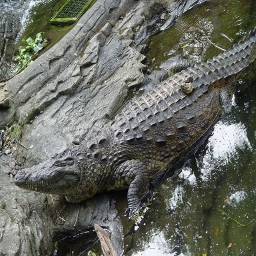
\includegraphics[width=80px,height=80px]{Figures/256.JPEG}
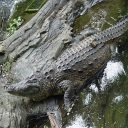
\includegraphics[width=80px,height=80px]{Figures/128.JPEG}
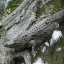
\includegraphics[width=80px,height=80px]{Figures/64.JPEG}
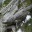
\includegraphics[width=80px,height=80px]{Figures/32.JPEG}
\caption{Едно и също изображение преоразмерено съответно на 256x256 128x128 64x64 и 32x32 пиксела}
\label{fig:example_sizes}
\end{figure}

\begin{longtable}{ | c | c | c | }
\hline
\textbf{Архитектура} & \textbf{Точност трен. данни} & \textbf{Точност тестови данни} \\ \hline \hline
Архитектура 0 & 87.47\% & 61.52\% \\ \hline
Архитектура 1 & 96.89\% & 62.41\% \\ \hline
Архитектура 1.1 & 94.20\% & 61.38\% \\ \hline
Архитектура 2 & 79.14\% & 63.38\% \\ \hline
Архитектура 2.1 & 72.20\% & 60.48\% \\ \hline
Архитектура 2.2 & 71.43\% & 59.10\% \\ \hline
\caption{Постигнати резултати при различните архитектури}
\label{tab:architectures_results}
\end{longtable}


\subsection{Експерименти върху Amazon cloud инстанция}
Поради много по-бързото изпълнение имаше възможност да се експериментира за повече класове, по-големи изображения и повече филтри. Използването на същите архитектури, но с по-големи изображения или повече филтри не доведе до увеличаване на точността. \ref{plot:plt_arch2_168px} Показва графика на точността по итерации. Постигнатите 60\% са по-малко от 63.38\% при размер на изображенията 64x64px.

\begin{figure}[H]
\centering
\begin{tikzpicture}
\begin{axis}[]
\addplot[
    color=blue,
    mark=square,
    ]
    coordinates {
    (1,	28.31)
    (2,	37.18)
    (3,	40.94)
    (4,	43.74)
    (5,	47.43)
    (6,	50.22)
    (7,	52.83)
    (8,	53.36)
    (9,	57.32)
    (10,58.78)
    (11,59.73)
    (12,62.20)
    (13,65.48)
    (14,68.88)
    (15,73.07)
    (16,76.38)
    (17,80.97)
    (18,84.35)
    (19,87.96)
    (20,92.20)
    (21,92.81)
    (22,94.15)
    (23,96.00)
    (24,96.10)
    (25,96.51)
    };
\addplot[
    color=red,
    mark=*
    ]
    coordinates {
    (1,	30.34)
    (2,	36.41)
    (3,	41.59)
    (4,	39.86)
    (5,	41.79)
    (6,	41.45)
    (7,	44.34)
    (8,	46.48)
    (9,	50.41)
    (10,51.59)
    (11,55.86)
    (12,54.21)
    (13,56.83)
    (14,56.48)
    (15,58.76)
    (16,57.66)
    (17,59.52)
    (18,60.97)
    (19,60.07)
    (20,58.48)
    (21,60.90)
    (22,60.62)
    (23,60.34)
    (24,58.83)
    (25,58.07)
    };
\legend{Точност за тренировъчните данни,Точност за тестовите данни}
\end{axis}
\end{tikzpicture}
\caption{Точност на \textbf{Архитектура 2} при \textbf{5 класа} и размер на изображенията \textbf{168x168px}}
\label{plot:plt_arch2_168px}
\end{figure}

\begin{figure}[H]
\centering
\begin{tikzpicture}
\begin{axis}[]
\addplot[
    color=blue,
    mark=square,
    ]
    coordinates {
    (1,	04.97)
    (2,	10.48)
    (3,	14.12)
    (4,	17.03)
    (5,	19.63)
    (6,	22.29)
    (7,	24.46)
    (8,	26.81)
    (9,	29.12)
    (10,31.69)
    (11,34.06)
    (12,36.34)
    (13,38.86)
    (14,40.88)
    (15,43.40)
    (16,45.48)
    (17,48.44)
    (18,50.56)
    (19,53.19)
    (20,55.42)
    (21,57.68)
    (22,60.18)
    (23,62.28)
    (24,64.62)
    (25,66.26)
    };
\addplot[
    color=red,
    mark=*
    ]
    coordinates {
    (1,	07.84)
    (2,	11.49)
    (3,	13.99)
    (4,	16.10)
    (5,	20.74)
    (6,	23.22)
    (7,	24.74)
    (8,	24.84)
    (9,	28.07)
    (10,28.75)
    (11,29.75)
    (12,30.83)
    (13,32.42)
    (14,32.76)
    (15,32.72)
    (16,33.32)
    (17,33.61)
    (18,34.33)
    (19,34.16)
    (20,34.54)
    (21,34.26)
    (22,34.71)
    (23,34.24)
    (24,34.75)
    (25,34.69)
    };
\legend{Точност за тренировъчните данни,Точност за тестовите данни}
\end{axis}
\end{tikzpicture}
\caption{Точност на \textbf{Архитектура 2} при \textbf{57 класа} и размер на изображенията \textbf{64x64px}}
\label{plot:plt_arch2_57cl}
\end{figure}


При опит за трениране върху всичките 57 класа с \textbf{Архитектура 2} една итерация отнема 243 секунди, което означава, че цялото изпълнение на 25 итерации отнема 1 час и 40 минути на инстанцията на Амазон. Тестът е направен с размер на изображенията 64x64 пиксела. За трениране за използвани 62920 изображения, а за валидиране - 15731. Постигнатата точност върху тренировъчните изображения е \textbf{66.26\%}, а върху тестовите \textbf{34.69\%}. \ref{plot:plt_arch2_57cl} показва прогреса на резултатите за всяка итерация.



\subsection{Проблемът с прекомерното нагаждане}

Както се вижда ясно на графиките с резултатите, при повечето архитектури е налице проблемът с прекомерното нагаждане (overfitting). При някои експерименти разликата в точността между тренировъчните и тестовите данни е над 30\%. Чрез леки промени в архитектурата и параметрите на конволюционните невронни мрежи тази разлика падна до 10-12\% (Архитектура 2.2), но на цената на по-лоша точност като цяло. Има и друго обяснение за този проблем и то е голямото разнообразие на изображенията. \ref{fig:different_images} показва 3 изображения от един и същи клас - алигатор, които се различават драстично. Именно огромните разлики в това какво точно е показано на картинките довежда до големите разлики между точността на тренировъчните и тестовите данни. Невронната мрежа успява успешно да класифицира първото и второто изображение, но не и третото.

\begin{figure}[H]
\centering
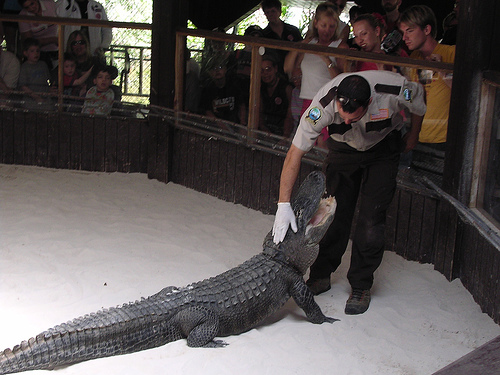
\includegraphics[width=110px,height=110px]{Figures/alig1.JPEG}
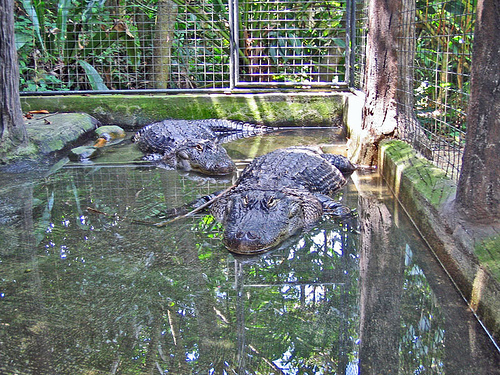
\includegraphics[width=110px,height=110px]{Figures/alig2.JPEG}
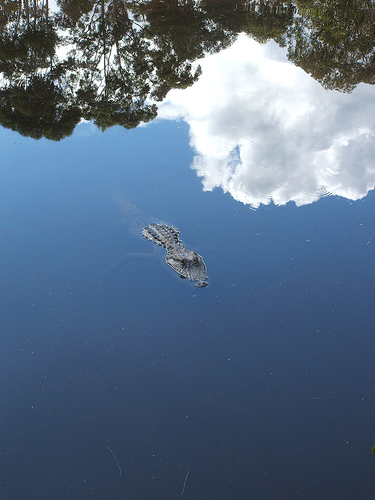
\includegraphics[width=110px,height=110px]{Figures/alig3.JPEG}
\caption{3 различни изображения от един и същи клас}
\label{fig:different_images}
\end{figure}






 
\chapter{Заключение}

\label{Chapter5}

%----------------------------------------------------------------------------------------

\section{Обобщение на изпълнението на началните цели}

Следва списък на началните цели и подробен анализ за постигнатите резултати относно всяка една от тях:
\begin{enumerate}
\item \textbf{Обзор на проблемната област}.\\
Областта е анализирана в детайли. Разгледани са различни приложения на класифицирането на изображения и бъдещето на тази сфера. В детайли са споменати някои от компаниите, които се занимават с това, както и по какво тяхното решение се отличава от останалите.

\item \textbf{Какви са условията (финансови, хардуерни и др.), за да построим класификатор с добра точност? Какво е добра точност и каква точност постигат готовите решения?}\\
Поради големият обем изображения, нужен за да се тренира добра конволюционна невронна мрежа хардуерът е от основно значение. Дори без да разполагаме с такъв можем да наемем cloud инстанция. С цел анализ, ускоряване на работата и постигане на по-добри резултати беше наета инстанция от Амазон. Тя успя да ускори работата 27-28 пъти в сравнение с локалната машина. Цената на услугата е в зависимост от ползването и варира: 25-40 цента на час за единично стартиране на инстанция и 90 цента на час за постоянна инстанция с гарантирана наличност. Амазон и други доставчици предлагат и по-мощни машини, за да удовлетворят всякакви цели.

Какво е добра точност е много относителен въпрос и зависи от начина, по който е зададен проблемът. Най-доброто известно решение до момента постига малко над 80\% точност за първият върнат клас (top 1). Ако проблемът се сведе до връщане на редица тагове за дадено изображение, то бихме могли да представим други мерки за точност, като например колко от върнатите тагове са адекватни за изображението и дали най-важните тагове са върнати от системата.

\item \textbf{Подбор на данни за обучение.}\\
Благодарение на ImageNet подборът на обучителни данни за целите на дипломната работа беше много бърз и лесен. Не така стоят нещата обаче, когато решението трябва да е глобално и да е обучено за всякакви теми и обекти. Някои компании изискват от клиентите си да предоставят тренировъчни изображения ако проблемът, който искат да се разреши е много специфичен.

\item \textbf{Реализация на прототип за класификация на изображения.}\\
Успешно беше реализиран прототип за класификация на изображения. За целите на дипломната работа са избрани класове, съставени от различни видове животни. Бяха изпробвани различни архитектури на конволюционни невронни мрежи и накрая трениран класификатор за разпонаване на 57 класа животни с 62920 тренировъчни изображения и 15731 тестови.

\item \textbf{Експерименти за оценка на точността на класификацията и възможностите за работа с големи данни.}\\
Направени са множество експерименти с 2 различни архитектури и техни разновидности (общо 5). Точността е измервана при всеки опит като 20\% от изображенията се заделят като тестови. С увеличение на броя на изображенията и с увеличение на техния размер времето за трениране и оценка нараства пропорционално. На наетата от Амазон инстанция при трениране на над 62000 изображения една итерация отнема 4 минути. На локалната машина тя би отнела над 1 час.

\item \textbf{Анализ на получените резултати.}\\
Резултатите са подробно анализирани. При 5 класа се постига точност над 63\% за тестовите и над 96\% за тренировъчните данни. При трениране върху 57 класа се постига точност над 34\% за тестовите и над 66\% за тренировъчните. При повечето опити е наличен проблемът за прекомерното нагаждане, който може да се обясни както с архитектурите и естеството на конволюционните невронни мрежи, така и с много разнообразните изображения от ImageNet.
\end{enumerate}

\section{Насоки за бъдещо развитие и усъвършенстване}
Изработената система може да бъде развивана и усъвършенствана в много насоки:

\begin{enumerate}
\item С цел постигане на по-добри резултати биха могли да се направят още множество експерименти, включително изпробване на други архитектури на невронната мрежа, промяна на хиперпараметрите, избор на нови тренировъчни изображения.
\item За по-бърза работа би могло да се наеме още по-добър хардуер и да се оптимизира процесът да използва повече от една видео карта. Това се позволява от интерфейса на библиотеката Tensorflow.
\item Системата би могла да се специализира в конкретна насока като например разпознаване на лица, идентифициране на туристически обекти или други.
\end{enumerate}
 

%----------------------------------------------------------------------------------------
%	BIBLIOGRAPHY
%----------------------------------------------------------------------------------------

\printbibliography[title={Референции},heading=bibnumbered]

%----------------------------------------------------------------------------------------

%----------------------------------------------------------------------------------------
%	APPLICATIONS
%----------------------------------------------------------------------------------------

\chapter{Приложения}

\label{Applications}

%----------------------------------------------------------------------------------------

\section{Приложение 1: Указание за инсталиране}

Предварителни изисквания:

\begin{itemize}
\item Linux базирана операционна система (софтуерът е тестван под Ubuntu 14.04 и Ubuntu 16.04).
\item Python версия 3 или по-нова.
\item Видео карта NVIDIA - интерфейсът CUDA разпознава само видео карти на NVIDIA. Ако видео картата не е NVIDIA софтуерът ще използва мощността на процесора и системата ще се забави значително.
\end{itemize}

Софтуерът използва Tensorflow, който от своя страна достъпва видео картата чрез CUDA. За целта трябва да се инсталират (Подробно описание: https://www.tensorflow.org/versions/r0.11/get\_started/os\_setup):

\begin{itemize}
\item CUDA toolkit 8.0
\item CuDNN v5
\item Tensorflow
\end{itemize}

Повечето модули, от които зависят програмите могат да се инсталират чрез pip. В ubuntu по подразбиране са инсталирани 2 версии на python: 2 и 3. За да се инсталира пакет с помощта на pip за python3 се използва pip3. Някои модули изискват повече права от други - трябва да се добави sudo пред pip3 за работа като администратор (su=super user). Python имплементацията зависи от следните модули:

\begin{itemize}
\item \textbf{os}: Използва се за записване и четене на файлове. Наличен е по подразбиране в python.
\item \textbf{random}: Използва се за генериране на произволни числа. Наличен е по подразбиране в python.
\item \textbf{pickle}: Използва се за сериализация (запазване на текущото състояние на обекти във файл). Наличен е по подразбиране в python. 
\item \textbf{time}: Използва се за работа с дати и часове. Наличен е по подразбиране в python.
\item \textbf{tarfile}: Използва се за работа с tar файлове. В такъв формат се свалят първоначално снимките от ImageNet. Наличен е по подразбиране в python.
\item \textbf{multiprocessing}: Използва се паралелна работа в повече от една нишка. Ускорява изтеглянето на изображенията и други процеси. Наличен е по подразбиране в python.
\item \textbf{pprint}: Използва се за принтиране на сложни структури от данни като речници и списъци. Наличен е по подразбиране в python.
\item \textbf{numpy}: Този модул е в основата на всички научни разработки, написани на python. Поддържа оптимизирани многомерни масиви, обработката им чрез функции от високо ниво и полезни практики от линейната алгебра. Ако не е наличен се инсталира с "pip install numpy".
\item \textbf{PIL}: Абревиатура на Python Imaging Library. Използва се за обработка на изображения. В контекста на програмата помага за преоразмеряването на всяко изображение в нужния формат. Инсталира се с "pip install pillow".

\item \textbf{h5py}: Използва се за запазване на вече обучен модел на невронна мрежа. Инсталира се последователно със следните 2 команди:

sudo apt-get install libhdf5\\
sudo pip3 install h5py
\item \textbf{keras}: Абстракция на работата с невронни мрежи. Използва Tensorflow. Инсталира се с "pip install keras". За повече информация: https://keras.io/\#installation.
\end{itemize}

\section{Приложение 2: Наръчник на потребителя}


Файловата организация е както следва:

\begin{itemize}
\item src
	\begin{itemize}
      \item data
      	\begin{itemize}
          \item bin\_generator.py
          \item image\_crawler.py
          \item imagenet\_metadata.py
        \end{itemize}
      \item main
      	\begin{itemize}
          \item common.py
          \item eval.py
          \item models.py
          \item retrain.py
          \item train.py
        \end{itemize}
      \item pretrained
      	\begin{itemize}
          \item audio\_conv\_utils.py
          \item imagenet\_utils.py
          \item inception\_v3.py
          \item resnet50.py
          \item test\_imagenet.py
          \item vgg16.py
          \item vgg19.py
          \item xception.py
        \end{itemize}
      \item config.py
    \end{itemize}
\item definitions.py
\item main.py
\end{itemize}


Единствената изходна точка на програмата е файлът \textbf{main.py} в директорията /image-recognition. След успешно стартиране на програмата, тя предоставя 4 опции на потребителя в следния диалог:\\
1. Image crawler\\
2. Bin Generator\\
3. Train\\
4. Eval\\
Choose what to do:

При избор на първата опция (\textbf{1. Image crawler}), програмата изтегля изображенията за 57-те класа в папка \_DATA в основната директория. Процесът може да отнеме време в зависимост от връзката към интернет и ядрата на компютъра. След изтегляне на всички изображения папката заема около 8.5 GB дисково пространство.

При избор на втората опция (\textbf{2. Bin Generator}), програмата създава папка в директорията \_MODELS с име текущата дата и час. Там добавя файлове с разширение .bin. Всеки един от тях съдържа информация за до 1000 изображения в удобен за четене формат. Броят на изображенията, за които е генерирана информация зависи от конфигурационния файл image-recognition/src/config.py.

При избор на третата опция (\textbf{3. Train}), програмата предоставя опция за избор на директория с генерирани .bin файлове. След избор, програмата тренира конволюционна невронна мрежа и запазва модела в същата папка в два файла: \_model.h5 и \_model.json. Освен това програмата принтира подробна информация за архитектурата на мрежата и точността при всяка итерация.

При избор на четвъртата опция (\textbf{4. Eval}), програмата отново предоставя опция за избор на директория с генериран модел. След избор, програмата оценява обучената невронна мрежа върху всеки един от класовете, за които е тренирана и изкарва статистика за точността.








%---------------------------------------------------------------------------------------- 

\end{document}  
